
\chapter{\uppercase{The Moment-Based Low-Order Equations}}
\label{chp:lo}

The LO equations are based on moments, i.e., integrals of the equations, to produce a
lower-dimensional system.  The equations incorporate extra parameters, referred to as
consistency terms, that allow for the equations to preserve the accuracy (particularly in
angle) of the HO solver, which is detailed in the next chapter. 
The formulation of the LO equations is similar to a discontinuous FE method.  Weighted
integrals of the equations are taken using weight functions that have local support. 
The equations are written with element-wise moments of $I$ and $T$ as
unknowns.  Leaving the solution in this form allows for use of information from a
previous HO solution to eliminate auxiliary unknowns from the equations. This is different
than a standard Galerkin or collocation FE
method~\cite{morel_ldtrt,morel_notes} where a
functional form of the solution is directly assumed. The final equations will have a
similar form to S$_2$ equations, but we have not used a collocation method in angle,
which should limit ray effects~\cite{morel_notes,lewis} in higher spatial dimensions.
The backward Euler time discretization is used throughout this section.
Chapter~\ref{sec:time} includes HO treatment of the radiation variables in the time
variable.

The remainder of this chapter is structured as follows: the general moments will be
derived and then the use of HO information to close the system in angle is discussed.
We then detail two separate spatial closures: a standard linear-discontinuous finite-element (LDFE)
method~\cite{morel_ldtrt} and the use of the HO solution to eliminate extra
spatial unknowns from the LO equations.  

\section{Forming the Space-Angle Moment Equations}

\subsection{LO Spatial mesh and Finite-Element Spatial Moments}

The LO equations are formulated over a FE mesh.  The domain for the $i$-th spatial
element (or cell) has support $x\in[x_{i-1/2},x_{i+1/2}]$ with width $h_i=x_{i+1/2} -
x_\il$ and cell center 
$x_i = x_\il + h_i/2$.  There is a total of $N_c$ elements, spanning the
spatial domain $0\leq x\leq X$.  For simplicity, this spatial mesh is fixed throughout the
simulation.  Mesh adaptation is only applied in the HO solver, where applicable.

\begin{figure}[H]
    \centering
    \begin{centering}
        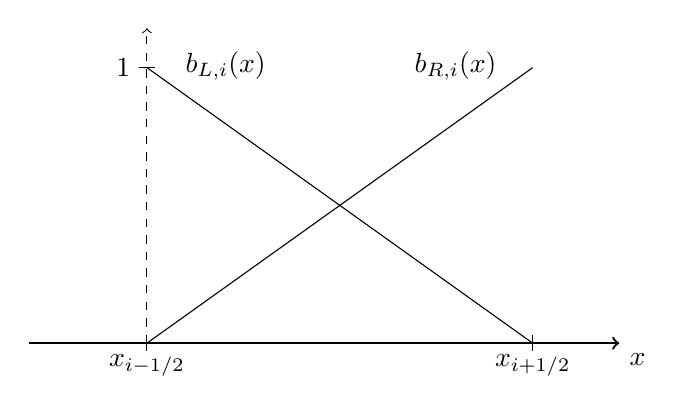
\begin{tikzpicture}[scale=1.0, every node/.style={transform shape}]
            \node at (10.7,4.0) {${1}$  };
            \draw (10.9,4.0) -- (11.1,4.0);
            \draw (11.0,0.4) -- (11.0,0.6) node[below, pos=0.4] {$x_{i-1/2}$};
            \draw (15.90,0.4) -- (15.90,0.6) node[below, pos=0.4] {$x_{i+1/2}$};
            \node at (14.92,4.02) {$b_{R,i}(x)$};
            \node at (12.0,4.02) {$b_{L,i}(x)$};
            \draw [thick,->] (9.5,0.5) -- (17.0,0.5) node[anchor=north west] {$x$};
            \draw [dashed,->] (11.0,0.5) -- (11.0,4.5);
            \draw (11.0,0.5) -- (15.90,4.0);
            \draw (15.90,0.5) -- (11.0,4.0);
        \end{tikzpicture}
    \end{centering}
    \caption{Illustration of linear finite element basis functions $b_{L,i}(x)$ and
    $b_{R,i}(x)$ for spatial element $i$.\label{fig:lin_fe}}
\end{figure}

The spatial moments are defined by integrals weighted with the standard linear finite element (FE)
interpolatory basis functions.  An illustration of the two linear FE basis functions for
the $i$-th element (or cell) is
given in Fig.~\ref{fig:lin_fe}.  The left basis function is defined as
\begin{equation}
    b_{L,i}(x)= \left\{\begin{matrix} \frac{\ds x_\ir - x}{\ds h_i} & x_\il \leq x \leq x_\ir
        \\ 0 &  \text{elsewhere}
    \end{matrix}\right.,
\end{equation}
corresponding to the node $x_\il$.
The right basis function is 
\begin{equation}
    b_{R,i}(x)= \left\{\begin{matrix} \frac{\ds x - x_\il}{\ds h_i} & x_\il \leq x \leq x_\ir
        \\ 0 & \text{elsewhere}
    \end{matrix}\right. ,
\end{equation}
corresponding to the node $x_\ir$. With these definitions, a local linear approximation to a
function $f$ can be formulated as $f(x)\simeq f_{L,i} b_{L,i}(x) + f_{R,i}
b_{R,i}(x),\quad x\in[x_{\il},x_{\ir}]$.\footnote{In literature the linear FE basis functions are
formally defined with support over two adjacent elements.  However, in our notation our 
functions only have non-zero support in element $i$. This accommodates our later
definition of moments and discontinuous unknowns.}

The spatial moments are defined by integrals over the each element, using the two
basis functions.  We use $\mom{\cdot}$ to indicate weighted integration over a
spatial element.  The spatial moments are
\begin{equation}\label{eq:x_moml}
\mom{\cdot}_{L,i} = \frac{2}{h_i} \int_{x_{i-1/2}}^{\xr} b_{L,i}(x) (\cdot) \dd x
\end{equation}
and
\begin{equation}\label{eq:x_momr}
\mom{\cdot}_{R,i} = \frac{2}{h_i} \int_{x_{i-1/2}}^{\xr} b_{R,i}(x) (\cdot) \dd x,
\end{equation}
where the factor of $2/h_i$ is a normalization constant.
In this notation $\mom{\phi}_{L,i}$ and
$\mom{\phi}_{R,i}$ represent spatial moments of the intensity over cell $i$, opposed
to $\phi_{L,i}$ and $\phi_{R,i}$, which represent the interior value of the linear
representation of $\phi(x)$ at $x_\il$ and $x_\ir$ within the cell. 

To simplify notation and discussion, we also define the slope and average moments over a
spatial cell.  The element-averaged scalar intensity is
\begin{equation}
    \phi_i = \frac{1}{h_i} \int_{\xl}^{\xr} \phi(x) \dd x
\end{equation}
and
\begin{equation}
    \phi_{x,i} = \frac{6}{h_i} \int_{\xl}^{\xr} \left(\frac{x-x_i}{h_i} \right)
    \phi(x) \dd x . 
\end{equation}
The linear representation over a cell can be written as $\phi(x) = \phi_i
+ 2\phi_{x,i}(x - x_i)/h_i^2$, for $x\in(\xl,\xr)$. 

\subsection{Definition of Angular Moments}

To reduce the angular dimensionality, positive and
negative half-range integrals of the angular intensity are taken.  The angular integrals
are denoted with a superscript as
\begin{equation}
    (\cdot)^\pm =  \pm\int_0^{\pm1} (\cdot) \dd \mu
\end{equation}
The half-range
integrals of $I$ are defined as $ \phi^+(x) = \int_0^{1} I(x,\mu)\, \dd \mu$ and $
\phi^-(x) =  \int_{-1}^{0} I(x,\mu) \,\dd
\mu$, respectively.  Thus, in terms of half-range quantities, the mean intensity is $\phi = \phi^- +
\phi ^+$.  It is noted that in this notation the flux is defined as
$J=J^-+J^+$, which is not the standard definition for the half-range fluxes, e.g.,
in~\cite{lewis}.

\subsection{Space-Angle Moments of the Radiation Transport Equation}

The LO radiation equations are formed by applying the space and angle moment operators to the
transport equation and performing algebraic manipulation.  We provide a detailed
derivation of the $L$ and $+$ radiation moment equation and state the final results for the
other moment operators.  The independent variables are often suppressed for some, or
all, of the dependent variables for compactness. 

First, the $L$ moment operator is applied to the time-discretized transport equation,
i.e., Eq.~\eqref{eq:trans_td}; application of integration by parts to the streaming term
of the resulting equation yields
\begin{multline}
    -\frac{2}{h_i}\mu I^{n+1}(x_{i-1/2},\mu) + \frac{2}{h_i^2}\int_{\xl}^{\xr} \mu I^{n+1}(x,\mu) \dd x
        +  \left(\sigma_{t,i}^{n+1}+\frac{1}{c \Delta t} \right)  
        \mom{I^{n+1}(x,\mu)}_{L,i} \\ -  \frac{\sigma_{s,i} }{2} \mom{\phi^{n+1}(x)}_{L,i} =
        \frac{1}{2} \mom{\sigma_{a,i}^{n+1} a c T^{n+1,4}(x)}_{L,i} +
  \frac{1}{c\Delta t}\mom{I^n(x,\mu)}_{L,i}.
\end{multline}
Here, the cross sections have been assumed constant over a cell and evaluated with
$T^{n+1}$. Now, the mean
intensity in the scattering term is expanded in terms of half-range unknowns.
The integral can be rewritten in terms of $L$ and $R$ moments by noting that $b_{L,i}(x) +
b_{R,i}(x) = 2/h_i$.  These substitutions are made, independent variables are suppressed, and the resulting equation is
multiplied by $h_i$ to produce
\begin{multline}
    -2\mu I_{i-1/2}^{n+1} + \mom{\mu I^{n+1}}_{L,i} + \mom{\mu I^{n+1}}_{R,i} 
        +  \left(\sigma_{t,i}^{n+1}+\frac{1}{c \Delta t} \right) h_i 
        \mom{I^{n+1}}_{L,i} \\-  \frac{\sigma_{s,i} h_i}{2} \left( \mom{\phi}_{L,i}^{n+1,+} +
  \mom\phi_{L,i}^{n+1,-}\right) = \frac{h_i}{2} \mom{\sigma_a^{n+1} a c T^{n+1,4}}_{L,i} +
  \frac{h_i}{c\Delta t}\mom{I^n}_{L,i},
\end{multline}
where $I_{i-1/2}(\mu)\equiv I(x_{i-1/2},\mu)$.
The resulting equation is integrated over the positive half range:
\begin{multline}\label{eq:spat_mom}
    -2\left({\mu} I_{i-1/2}^{n+1}\right)^+ + \mom{\mu I^{n+1}}^+_{L,i} + \mom{\mu
        I^{n+1}}^+_{R,i} 
        +  \left(\sigma_{t,i}^{n+1}+\frac{1}{c \Delta t} \right) h_i 
  \mom{\phi}_{L,i}^{n+1,+} \\-  \frac{\sigma_{s,i} h_i}{2} \left( \mom{\phi}_{L,i}^{n+1,+} +
  \mom\phi_{L,i}^{n+1,-}\right) = \frac{h_i}{2} \mom{\sigma_a^{n+1} a c T^{n+1,4}}_{L,i} +
  \frac{h_i}{c\Delta t}\mom{\phi}_{L,i}^{n,+}.
\end{multline}

\subsection{The Angular Consistency Terms}
\label{sec:ang_cons}

Now, algebraic manipulations are performed on the streaming terms to produce face and
volume averages of $\mu$, weighted by the intensity.  Each term in the streaming
term of Eq.~\eqref{eq:spat_mom} is multiplied by a factor of unity, with the desired unknown appropriate to each term
in the numerator and denominator, as in~\cite{wolters}.  Temporarily dropping the time
index for clarity, the manipulations applied to
the streaming term are as follows:
    \begin{align} \label{eq:line1}
        {\displaystyle \left \langle \mu \pderiv{I}{x} \right \rangle_L^+ } & = 
        -\frac{\ds2}{\ds h_i} \left(\mu I_{i-1/2}\right)^+ + \frac{\ds 1}{\ds h_i}\left[
    \mom{\mu I}_{L,i}^+ + \mom{\mu I}_{R,i}^+ \right] \\
        & =  
        -\frac{\ds2}{\ds h_i} \left(\mu I_{i-1/2}\right)^+
        \! \frac{\ds(I_{i-1/2})^+}{\ds(I_{i-1/2})^+}  \;    + \frac{\ds 1}{\ds h_i}\left[ \;
        \mom{\mu I}_{L,i}^+ \! \frac{\ds\mom{I}_{L,i}^+}{\ds\mom{I}_{L,i}^+} \; + \; \mom{\mu
        I}_{R,i}^+ \! \frac{\ds\mom{I}_{R,i}^+}{\ds\mom{I}_{R,i}^+} \right] \\
        & =  -\frac{\ds2}{\ds h_i} \left\{ {\frac{\ds \left( \mu I
            \right)^+_{i-1/2} }{\ds\phi^+_{i-1/2}}} \right\}
            \phi^+_{i-1/2} + \frac{\ds 1}{\ds h_i} \left[ \left\{ {\frac{\ds\mom{\mu
        I}_{L,i}^+}{\ds\mom{\phi}_{L,i}^+}} \right \} \mom{\phi}_{L,i}^+  +
        \left\{ {\frac{\ds\mom{\mu I}_{R,i}^+}{\ds\mom{\phi}_{R,i}^+}} \right\}
    \mom{\phi}_{R,i}^+ \right]
    \end{align}
The ratios in braces are what we will formally define as \emph{angular consistency terms}.
These nonlinear functionals are approximated by the HO solver, similar to the approach
in~\cite{wolters}.  The angular consistency
term for the $L$ and $+$ moments is defined as
\begin{equation}\label{eq:ang_cons_vol}
    \cur{{\mu}}_{L,i}^{n+1,+} \equiv \frac{\mom{\mu I^{n+1}}_{L,i}^+}{\mom{I^{n+1}}_{L,i}^+} =  \frac{
{\displaystyle \frac{2}{h_i}} \int\limits_0^1 \int\limits_\xl^\xr \mu \, b_{L,i}(x)
I^{n+1}(x,\mu) \dd x \dd \mu } 
{{\displaystyle \frac{2}{h_i}} \int\limits_0^1 \int\limits_\xl^\xr \, b_{L,i}(x)
I^{n+1}(x,\mu) \dd x \dd \mu } .
\end{equation}
The consistency terms on the face represent averaging at a point, with a similar
definition as
\begin{equation}\label{eq:ang_cons_face}
    {\mu}_{i+1/2}^{+} \equiv \frac{\left(\mu I_{i+ 1/2}\right)^+}{\phi_{i+1/2}^+}=  \frac{
        {\displaystyle \int\limits_0^1 \mu I(x_{i+1/2},\mu) \dd \mu }} 
        {{\displaystyle \int\limits_0^1 I(x_{i+1/2},\mu) \dd \mu }} \;.
\end{equation}
There are analogous definitions for the $R$ and $-$ moments, e.g.,
\begin{equation}\label{eq:ang_cons_vol}
    \cur{{\mu}}_{R,i}^{n+1,-} \equiv \frac{\mom{\mu I^{n+1}}_{R,i}^-}{\mom{I^{n+1}}_{R,i}^-} =  \frac{
        {\displaystyle \frac{2}{h_i}} \int\limits_{-1}^0 \int\limits_\xl^\xr \mu \, b_{R,i}(x)
I^{n+1}(x,\mu) \dd x \dd \mu } 
{{\displaystyle \frac{2}{h_i}} \int\limits_{-1}^0 \int\limits_\xl^\xr \, b_{R,i}(x)
I^{n+1}(x,\mu) \dd x \dd \mu } .
\end{equation}
Substitution of Eq.~\eqref{eq:ang_cons_vol}~and~\eqref{eq:ang_cons_vol} simplifies
moments of the streaming
term for the $L$ and $+$ operators:
\begin{equation}\label{eq:stream_mom}
        {\displaystyle \left \langle \mu \pderiv{I}{x} \right \rangle_L^+ } = 
        -\frac{\ds2}{\ds h_i} \mu_{i-1/2}^+ I_{i-1/2}^+ + \frac{1}{h_i}\left[
        \cur{\mu}_{L,i}^+ \mom{\phi}^+_{L,i} + \cur{\mu}_{R,i}^+ \mom{\phi}_{R,i}^+
    \right]
\end{equation}
It is noted that this expression does not contain a cross section in the denominator,
such as in the variable Eddington factor approach~\cite{ferguson}, eliminating 
issues in a void where $\sigma_t=0$.


\subsection{The Exact Radiation Moment Equations}

A final form of the moment equation resulting from application of the $L$ moment and
positive half-range integral is obtained by substitution of 
Eq.~\eqref{eq:stream_mom} into Eq.~\eqref{eq:spat_mom}:
\begin{multline}\label{eq:exact_lmomp}
    -2{\mu}_{i-1/2}^{n+1,+} \phi_{i-1/2}^{n+1,+} + \cur {\mu}_{L,i}^{n+1,+}
  \mom{\phi}_{L,i}^{n+1,+}
  +  \cur\mu_{R,i}^{n+1,+}
  \mom{\phi}_{R,i}^{n+1,+} +  \left(\sigma_{t,i}^{n+1}+\frac{1}{c \Delta t} \right) h_i 
  \mom{\phi}_{L,i}^{n+1,+} \\-  \frac{\sigma_{s,i} h_i}{2} \left( \mom{\phi}_{L,i}^{n+1,+} +
  \mom\phi_{L,i}^{n+1,-}\right) = \frac{h_i}{2} \mom{\sigma_a^{n+1} a c T^{n+1,4}}_{L,i} +
  \frac{h_i}{c\Delta t}\mom{\phi}_{L,i}^{n,+},
\end{multline}
The other radiation moment equations are derived analogously.  
Pairwise application of the $L$ and $R$ basis
moments with the $+$ and $-$ half-range integrals to Eq.~\eqref{eq:trans_td} 
ultimately yields four moment
equations per cell.  The equation for the $R$ and $+$ moment is
\begin{multline}\label{eq:exact_rmomp}
    2{\mu}_{i+1/2}^{n+1,+} \phi_{i+1/2}^{n+1,+} - \cur {\mu}_{L,i}^{n+1,+}
  \mom{\phi}_{L,i}^{n+1,+}
  -  \cur\mu_{R,i}^{n+1,+}
  \mom{\phi}_{R,i}^{n+1,+} +  \left(\sigma_{t,i}^{n+1}+\frac{1}{c \Delta t} \right) h_i 
  \mom{\phi}_{R,i}^{n+1,+} \\-  \frac{\sigma_{s,i} h_i}{2} \left( \mom{\phi}_{R,i}^{n+1,+} +
  \mom\phi_{R,i}^{n+1,-}\right) = \frac{h_i}{2} \mom{\sigma_a^{n+1} a c T^{n+1,4}}_{R,i} +
  \frac{h_i}{c\Delta t}\mom{\phi}_{R,i}^{n,+},
\end{multline}
The equations for the negative half-range moment are identical to the above with the
negative half-range integrals replacing the positive where applicable.  Explicitly,
\begin{multline}\label{eq:exact_lmomm}
    -2{\mu}_{i-1/2}^{n+1,-} \phi_{i-1/2}^{n+1,-} + \cur {\mu}_{L,i}^{n+1,-}
  \mom{\phi}_{L,i}^{n+1,-}
  +  \cur\mu_{R,i}^{n+1,-}
  \mom{\phi}_{R,i}^{n+1,-} +  \left(\sigma_{t,i}^{n+1}+\frac{1}{c \Delta t} \right) h_i 
  \mom{\phi}_{L,i}^{n+1,-} \\-  \frac{\sigma_{s,i} h_i}{2} \left( \mom{\phi}_{L,i}^{n+1,+} +
  \mom\phi_{L,i}^{n+1,-}\right) = \frac{h_i}{2} \mom{\sigma_a^{n+1} a c T^{n+1,4}}_{L,i} +
  \frac{h_i}{c\Delta t}\mom{\phi}_{L,i}^{n,-}
\end{multline}
and
\begin{multline}\label{eq:exact_rmomm}
    2{\mu}_{i+1/2}^{n+1,-} \phi_{i+1/2}^{n+1,-} - \cur {\mu}_{L,i}^{n+1,-}
  \mom{\phi}_{L,i}^{n+1,-}
  -  \cur\mu_{R,i}^{n+1,-}
  \mom{\phi}_{R,i}^{n+1,-} +  \left(\sigma_{t,i}^{n+1}+\frac{1}{c \Delta t} \right) h_i 
  \mom{\phi}_{R,i}^{n+1,-} \\-  \frac{\sigma_{s,i} h_i}{2} \left( \mom{\phi}_{R,i}^{n+1,+} +
  \mom\phi_{R,i}^{n+1,-}\right) = \frac{h_i}{2} \mom{\sigma_a^{n+1} a c T^{n+1,4}}_{R,i} +
  \frac{h_i}{c\Delta t}\mom{\phi}_{R,i}^{n,-},
\end{multline}
Ultimately, the two half-ranges will be treated differently when the equations are closed
spatially.

\subsection{Material Energy Equations}

To derive the LO material energy equations, an approximation must be introduced to relate
$T(x)$ and $T^4(x)$ within a cell.  We represent $T(x)$ spatially 
with a LDFE trial space, i.e., $ T(x) \simeq T_{L,i} b_{L,i}(x) + T_{R,i} b_{R,i}(x),\quad x\in(x_{i-1/2},x_\ir)$.
This trial space will ensure preservation of the equilibrium
diffusion limit and limit artificial propagation of energy across the system~\cite{teleportation}. 
Similarly, the emission term is represented in the material and radiation equations with the LDFE
interpolant $T^4(x)\simeq T_{L,i}^4 b_{L,i}(x) + T_{R,i}^4 b_{R,i}(x)$.   The $L$ and $R$ spatial moments are taken of the material
energy equations, and the LDFE representations for $T(x)$ and $\sigma_a a c T^4(x)$ are used to
simplify the spatial integrals. The final LO material energy
 equation resulting from application of the $L$ moment is
 \begin{multline}\label{eq:lo_mat_dis1}
     \frac{\rho_i c_{v,i}}{\Delta t}\left[ \left(\frac{2}{3}T_{L,i} + \frac{1}{3}T_{R,i}
        \right)^{n+1} - \left(\frac{2}{3}T_{L,i} + \frac{1}{3}T_{R,i}
    \right)^{n} \right]  + \sigma_{a,i}^{n+1} \left( \mom{\phi}_{L,i}^+ +
    \mom{\phi}_{L,i}^- \right)^{n+1} \\ = \sigma_{a,i}^{n+1}a c
\left( \frac{2}{3} T_{L,i}^4 + \frac{1}{3}T_{R,i}^4
        \right)^{n+1}.
\end{multline}
The equation for the $R$ moment is
 \begin{multline}\label{eq:lo_mat_dis2}
     \frac{\rho_i c_{v,i}}{\Delta t}\left[ \left(\frac{1}{3}T_{L,i} + \frac{2}{3}T_{R,i}
        \right)^{n+1} - \left(\frac{1}{3}T_{L,i} + \frac{2}{3}T_{R,i}
    \right)^{n} \right]  + \sigma_{a,i}^{n+1} \left( \mom{\phi}_{R,i}^+ +
    \mom{\phi}_{R,i}^- \right)^{n+1} \\ = \sigma_{a,i}^{n+1}a c
\left( \frac{1}{3} T_{L,i}^4 + \frac{2}{3}T_{R,i}^4
        \right)^{n+1}.
\end{multline}
Cross sections have been assumed constant over each element, evaluated at the
average temperature within the element, i.e., $\sigma_{a,i}^{n+1} =
\sigma_{a,i}([T^{n+1}_{L,i}+T^{n+1}_{R,i}]/2)$.
Because the material energy balance equation
 only contains angularly integrated quantities, there is no need to take angular
 moments of the above equations.  


\section{Closing the LO Equations in Space and Angle}
\label{sec:closure}

At this point, the LO equations have too many unknowns: the relation between the volume
and face averaged quantities and the angular consistency parameters are not known a
priori. The HO solution is used to eliminate the consistency parameters and other
approximations are used to eliminate the extra spatial unkonwns from the equations.
The six degrees of freedom (DOF) over each cell $i$ are the four moments $\mom{\phi}_{L,i}^+$,
$\mom{\phi}_{R,i}^+$, $\mom{\phi}_{L,i}^-$, and $\mom{\phi}_{R,i}^-$ and the two
spatial edge values $T_{L,i}$ and $T_{R,i}$.  After closure, the four radiation and two material
energy equations define a system of equations for the six DOF, coupled spatially through
the streaming term.  

Before introducing the additional closures, we emphasize that at this point the only spatial or
angular approximations to the radiation  moment equations are an LDFE
representation for $T^4(x)$ and cell-averaged cross sections; these moment equations are exact with
respect to the chosen time discretization and these approximations.  The material energy
equations, as well as the emission source, required an approximation of LDFE in space for $T(x)$ and $T^4(x)$.  Some
approximation is always necessary
to relate $T$ and $T^4$.

\subsection{Angular Closure}

The angular consistency
parameters (e.g., Eq.~\eqref{eq:ang_cons_vol} and~\eqref{eq:ang_cons_face}) are not known a priori. 
A lagged estimate of $I^{n+1}$ from the previous HO solve is
used to estimate the angular consistency parameters. In the HOLO algorithm, the equations for LO unknowns at iteration $k+1$ use consistency parameters
computed using the latest HO solution $\tilde{I}^{n+1,k+1/2}$
as an approximation for $I^{n+1}(x,\mu)$, e.g.,
\begin{equation}\label{eq:ang_cons_vol}
    \cur{{\mu}}_{L,i}^{n+1,+} \simeq \frac{\mom{\mu
    \tilde I_{HO}^{n+1,k+1/2}}_{L,i}^+}{\mom{\tilde I_{HO}^{n+1,k+1/2}}_{L,i}^+} =  \frac{
{\displaystyle \frac{2}{h_i}} \int\limits_0^1 \int\limits_\xl^\xr \mu \, b_{L,i}(x)
\tilde I^{n+1,k+1/2}_{HO}(x,\mu) \dd x \dd \mu } 
{{\displaystyle \frac{2}{h_i}} \int\limits_0^1 \int\limits_\xl^\xr \, b_{L,i}(x)
\tilde I^{n+1,k+1/2}_{HO}(x,\mu) \dd x \dd \mu } .
\end{equation}
We evaluate these terms using quadrature based
on the LDFE functional representation $\tilde I_{HO}(x,\mu)$ provided by the HO solution.

\subsection{LDFE Spatial Closure}

After approximating the angular consistency terms in the time-discretized LO moment equations, 
a equation relating the spatial moments and outflow face values is
needed to eliminate the final auxiliary unknowns, i.e., a spatial closure.
We will eliminate the face terms to produce equations exclusively the desired moment
unknowns.  Several closures were investigated.  The simplest closure
is a linear-discontinuous (LD) spatial closure with the usual upwinding
approximation~\cite{morel_ldtrt}.  A closure based on the HO solution is discussed in
Sec.~\ref{sec:spat_clos}.  Because there are no derivatives of $T$ in Eq.~\eqref{eq:mat_td}, there is no need
to define $T$ on the faces in Eq.~\eqref{eq:lo_mat_dis1} and Eq.~\eqref{eq:lo_mat_dis2};
only moments of $\phi$ appear in the material energy
equations, thus they are fully defined at this point and require no additional spatial
closure.  

Now, the LDFE closure is applied to the radiation moment equations for the case of
positive flow (i.e., Eq.~\eqref{eq:exact_lmomp} and~\eqref{eq:exact_rmomp}). The LD
closure over for the $i$-th cell and positive $\mu$ 
is illustrated in Fig.~\ref{fig:ld_il}.  The face terms $\mu_{i-1/2}$ and $\phi_{i-1/2}$
are upwinded from the previous cell $i-1$ or from a boundary condition; the terms
at $x_{i+1/2}$ are linearly extrapolated, computed using the $L$ and $R$ basis
moments.  The linear approximation $\phi^+(x)=b_{L,i}(x)\phi^+_{L,i} +
b_{R,i}(x)\phi^+_{R,i}$, for $x\in(\xl,\xr]$, is substituted into the definition for
the moments (i.e., Eq.~\eqref{eq:x_moml}~and~\eqref{eq:x_momr}) and solved for the LD edge value
$\phi_{i,R}^+$; The resulting outflow relation for positive flow is $\phi^+_{i+1/2} \equiv \phi_{i,R}^+ = 2\mom{\phi}_{R,i}^+ -
\mom{\phi}_{L,i}^+$; the LD closure for the negative half range produces $\phi^-_{i-1/2} = 2\mom{\phi}_{L,i}^- -
\mom{\phi}_{R,i}^+$. The $L$ moment and positive half-range equation with the LD closure and upwinding is
\begin{multline} 
    -2{\mu}_{i-1/2}^{n+1,+} \left(2\mom{\phi}_{R,i-1}^{n+1,+} -   \mom{\phi}_{L,i-1}^{n+1,+}      \right) + \cur {\mu}_{L,i}^{n+1,+}
  \mom{\phi}_{L,i}^{n+1,+}
  +  \cur\mu_{R,i}^{n+1,+}
  \mom{\phi}_{R,i}^{n+1,+}\\ +  \left(\sigma_{t,i}^{n+1}+\frac{1}{c \Delta t} \right) h_i 
  \mom{\phi}_{L,i}^{n+1,+} -  \frac{\sigma_{s,i} h_i}{2} \left( \mom{\phi}_{L,i}^{n+1,+} +
  \mom\phi_{L,i}^{n+1,-}\right)\\  = \frac{h_i}{2} \mom{\sigma_a^{n+1} a c T^{n+1,4}}_{L,i} +
  \frac{h_i}{c\Delta t}\mom{\phi}_{L,i}^{n,+}.
\end{multline}
Similar equations can be derived for the other directions and moments, fully defining the radiation
equations.   The closed equations are equivalent in numerical complexity to an LDFE
discretization of the S$_2$ equations~\cite{morel_ldtrt,lewis}, but with different quadrature points on the face
and interior.

\begin{figure}[H]
    \centering
    {\resizebox{0.5\textwidth}{!}{
        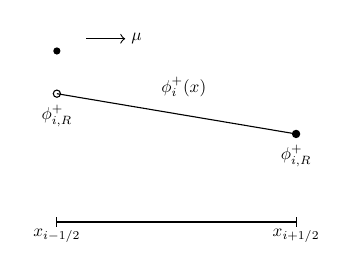
\begin{tikzpicture}[scale=0.62, every node/.style={transform shape}]
            \draw (1.0,4.0) node[fill,circle,inner sep=0pt,minimum
            size=4.2pt] {};
            \draw [->] (1.6,4.25) -- (2.4,4.25) node[anchor=west] {$\mu$};
            \draw (1.0,0.4) -- (1.0,0.6) node[below, pos=0.4] {$x_{i-1/2}$};
            \draw (5.90,0.4) -- (5.90,0.6) node[below, pos=0.4] {$x_{i+1/2}$};
            \node at (3.6,3.26) {$\phi_i^+(x)$};
            \node[anchor=north] at (5.9,2.2) {${\phi^+_{i,R}}$};
            \draw [thick] (1.0,0.5) -- (5.9,0.5) node[anchor=north west] {};
            \filldraw[color=black, fill=white] (1,3.1250) circle (2.1pt);
            \draw (1.0,3.125) -- (5.90,2.30);
            \node[anchor=north] at (1.0,3.025) {${\phi^+_{i,R}}$};
            \filldraw (5.9,2.30) circle (2.1pt);
        \end{tikzpicture}
    }}
    \caption{Linear discontinuous trial space for half-range mean intensity and $\mu>0$,
        in LO equations.\label{fig:ld_il}}
\end{figure}

Note that we have chosen to leave $\mu_{i-1/2}^{n+1,+}$ as a value to be estimated from the HO solver,
which is more conducive to the HO spatial closures described in
Sec.~\ref{sec:spat_clos}.
Alternatively, the spatial closure could be introduced before performing the algebraic
manipulation to form consistency terms (e.g., into Eq.~\eqref{eq:line1}).  This would produce only volume-weighted consistency
terms in the equations.  




\subsection{Boundary Conditions}

For all spatial closures, the specified incident angular intensity is
incorporated into the upwinding term of the appropriate radiation moment equation.   At the left
boundary, the upwinded current is known, so for that $L$ moment equation
\begin{equation}
    \mu_{1/2}^+ \phi_{1/2}^+ = \int_{0}^1 \mu I^{inc,+}(\mu) \dd \mu,
\end{equation}
where $I^{inc,+}(\mu)$ is the specified incident angular intensity at the left boundary.  For all
results in this work, only isotropic incident intensities were considered.
A similar expression is derived for the right boundary.
  For S$_2$-equivalent LO solves, i.e., all consistency
terms are $\pm 1/\sqrt{3}$, the half-range flux in the above equation is renormalized by
multiplying the term in the moment equations by $2/\sqrt{3}$ to produce accurate solutions~\cite{morel_notes}.     


\section{Newton's Method for LO Equations}
\label{sec:newton_overview}

Summation over all cells of the closed equations forms a global system of coupled equations.
The equations are nonlinear due to the Planckian emission source.  
We have used a local Newton's method to solve the nonlinear system, based on a standard linearization of the Planckian source with cross
sections evaluated at temperatures from the previous iteration, as described
in~\cite{morel_ldtrt}.  A derivation of the LO Newton equations is given
in~\ref{app:lo_newton}.

The equations for each half-range are coupled together via scattering.  
In one spatial dimension, the scattering terms can be included in the discrete system
matrix and directly inverted.  We consider an alternative iterative solution method that
could be more easily extended to higher spatial dimensions in Sec.~\ref{sec:dsa}.
For the direct solution method, isotropic scattering,
including effective scattering terms from the linearization, are included in the system matrix. The system
matrix is an asymmetric, banded matrix with a band width of seven and is inverted
directly. 
Newton iterations are repeated until $\phi^{n+1}(x)$ and $T^{n+1}(x)$ are converged
to a desired relative tolerance.  Convergence in the Newton iterations is calculated using the spatial $L_2$
norm of the change in $\phi^{n+1}(x)$ and $T^{n+1}(x)$, relative to the norm of each
solution.  

In certain problems, the nonlinearities of the system can lead to divergence of the Newton
iterations.  This is often the result of taking relatively large time steps for problems with large
values of $\sigma_a$ and small values of $\rho c_v$.  To prevent divergence, a damped
Newton method~\cite{damped_newton} can be used, at the cost of increased numbers of iterations.  For a
damped Newton's method, the estimated change in the solution between iterations is multiplied by a factor $\xi\in(0,1)$, where $\xi$ is referred to as the damping factor.
Sufficient reduction of the change in solutions between iterations will allow iterations
to continue converging, by ensuring the solution remains with the domain of convergence.  
The details of modifying the Newton iterations in this work to include a damping factor are given in
App.~\ref{app:damped_newton}.  For simplicity, a fixed value of $\xi$ was used for all
iterations in problems where damping was found to be necessary.

%Application of the first order Taylor expansion in time of the
%gray emission source, about some temperature $T^*$ at some
%time near $t^{n+1}$ gives
%\begin{equation}\label{new_planck}
%    \sigma_a^* a c T^{4,n+1} \simeq \sigma_a^* a c \left[T^{*4} + (T^{n+1} - T^*) 4T^{*3} \right]
%\end{equation}
%where the superscript $*$ denotes evaluation at $T^*$. A spatially discretized form
%of this expression is substituted
%into the emission term in the discretized material
%energy equations, e.g., Eq.~\eqref{lo_mat_dis}.  This allows for the material energy
%equation to be eliminated from the system, introducing effective scattering and
%emission sources into the right hand side
%of the LO radiation equations. This defines four linear equations for the four remaining radiation unknowns. 
%Once these linear equations have been solved for $\phi^{n+1}$, a new estimate of
%$T^{n+1}$ can be determined using the same linearization (Eq.~\eqref{new_planck}) to
%conserve the total energy.  This estimate of $T^{n+1}$ can now be used as $T^*$ to form a more
%accurate linearization of the emission source. 

\section{Fix-ups for Negative Solutions with LDFE Closure}
\label{sec:ldfe_fixups}

The linear-discontinuous (LD) closure with upwinding is not strictly positive.  In particular, for
optically thick cells with a steep intensity gradient, the linear representations for
$\phi(x)$ and $T(x)$ can go below the floor temperature or negative. 
The floor temperature $T_{\min}$ is defined as the initial
temperature of the material and radiation in problems where boundary sources are
applied at each of the boundaries.  In such problems the radiation and material should
continue to heat on the interior of the domain, and should physically not fall below
the initial temperature. 
Negative values of intensity can propagate to adjacent cells. In thick regions of
TRT problems, reasonably fine spatial cells can still be on the order of millions of mean
free paths; negative values with an LD representation are unavoidable in practice for
such cells and mesh refinement is of minimal use. 

Typically, for a standard LDFE Galerkin spatial discretization,
the equations are lumped to produce a discretization that is strongly resistant to
negative values (for 1D)~\cite{morel_ldtrt}.
However, standard FE lumping
procedures would introduce difficulties in computing the consistency terms from the
HO solution.  
 Alternatively, we have derived a modified spatial closure that produces
unknowns equivalent to those from a lumped LD method in 1D.
The $L$ and $R$ moments are defined the same as before,
preserving the average within a cell, but the relation between the moments and
the outflow is modified. 
In the lumping-equivalent closure, the outflows are defined as
\begin{align}
    \phi_{i+1/2}^+ &= \mom{\phi}_{i,R}^+ \\
    \phi_{i-1/2}^- &= \mom{\phi}_{i,L}^-. 
\end{align}
The system is then fully defined with upwinding and the assumption of a linear relationship on
interior of the element.  This modified closure produces a linear
representation that preserves zeroth moment, but the relation between the slope of the line and the 
first spatial moment has been modified.  Because the basis functions $b_{R,i}(x)$ and $b_{L,i}(x)$ are strictly
positive, the outflows tends to be positive. Strong sources and gradients can still lead to
negativities at the edges of the LD representation.  Details on the
derivation of this relation are in Appendix~\ref{app:lo_mom_relations}. 
The lumping closure was optionally applied in all cells or only in cells where negative
 intensities occur.  

For simplicity,
we also lump the emission source and temperature terms in the equations following the
standard procedure~\cite{morel_ldtrt}.  For example, the lumped version of Eq.~\eqref{eq:lo_mat_dis1}
is
\begin{equation}\label{eq:lumped_mat}
     \frac{\rho_i c_{v,i}}{\Delta t}\left(T_{L,i}^{n+1} - T_{L,i}^{n}\right)  + \sigma_{a,i}^{n+1} \left( \mom{\phi}_{L,i}^+ +
    \mom{\phi}_{L,i}^- \right)^{n+1} \\ = \sigma_{a,i}^{n+1}a c
    \left( T_{L,i}^{n+1}\right)^4
    \end{equation}
noting that no modification was made to the radiation moment term in this equation.  It was found that
lumping the temperature equations generally produced more robustness than exclusively
modifying the spatial closure, but is not necessary for all problems.

We also investigated an alternative closure of the equations based on energy conservation
and forcing the appropriate edge value to be the floor value.
The equations within cells that produce a negativity are modified to ensure the edge
intensities are not below the floor temperature, and energy balance is
conserved.  This fixup is only applied in cells where a intensity has occured during
inversion of the LO streaming plus removal operator.  For example, if $\phi^+_{R,i}$
is found to be negative, the modified equations (for the positive half range) in that cell are
the balance equation, i.e., 
\begin{multline}\label{eq:floor_outflow}
    -{\mu}_{i-1/2}^{n+1,+} \left(2\mom{\phi}_{R,i-1}^{n+1,+} -   \mom{\phi}_{L,i-1}^{n+1,+}      \right) +
    {\mu}_{i+1/2}^{n+1,+} \left(2\mom{\phi}_{R,i}^{n+1,+} -
    \mom{\phi}_{R,i}^{n+1,+}\right) \\       
   +  \left(\sigma_{t,i}^{n+1}+\frac{1}{c \Delta t} \right)
  \frac{h_i}{2} \left(\mom{\phi}_{L,i}^{n+1,+} + \mom{\phi}_{R,i}^{n+1,+}\right) -  \frac{\sigma_{s,i} h_i}{4} \left( \mom{\phi}_{L,i}^{n+1} +
  \mom\phi_{R,i}^{n+1}\right)\\  = \frac{h_i}{4} \sigma_{a,i}^{n+1} a c \left(
    \mom{T^{n+1,4}}_{L,i} + \mom{T^{n+1,4}}_{R,i} \right) +
  \frac{h_i}{2c\Delta t}\left(\mom{\phi}_{L,i}^{n,+} + \mom{\phi}_{R,i}^{n,+}\right)
\end{multline}
and the closure equation, i.e., 
\begin{equation}\label{eq:clos_outflow}
    2\mom{\phi}_{i,R}^+ - \mom{\phi}_{i,L}^+ = T_{\min}.
\end{equation}

Because our solution method directly inverts the LO system,
negative edge intensities must be detected, the fix-up applied locally to all elements and half-ranges
where necessary, and then that Newton solve
repeated.  In practice, this flooring procedure was observed to produce positive answers, but was not as robust as performing
lumping in all cells.  In general, as the time step size is increased, this fixup led to the Newton
solve diverging (i.e., damping is required to converge the iterations), more rapidly than if lumping was
used for all cells.  A similar effect was observed in some problems when attempting to only lump the
equations in cells where negativities were observed and resolving that Newton step.


\section{Accuracy in the Equilibrium Diffusion Limit}
\label{sec:edl_overview}

In our standard LO scheme, the
LO equations use an LDFE representation for the temperature and the uld preserve the equilibrium diffusion limit.  In this limit, the MC HO
solution will estimate angular consistency terms associated with an isotropic intensity,
based on a spatially LD emission source.  This produces equations that are equivalent to
the S$_2$ equations, but with quadrature points defined by $\pm 1/2$.  Because the spatial closure produces equations that are equivalent to an LDFE
solution to the S$_2$ equations, we expect the equations to preserve the equilibrium diffusion
limit, which is known to preserve the EDL based on discrete asymptotic analysis~\cite{morel_ldtrt}.
